\section{Исследовательский раздел}

\par В данном разделе будет исследована эффективность разработанного комбинированного метода прогнозирования временных рядов при различных сочетаниях используемых моделей. На основе полученных значений будет произведен сравнительный анализ комбинаций разработанных моделей. По результатам проведенного исследования будут сделаны выводы о точности предсказаний гибридной модели.

\subsection{Эффективность предсказаний}

\textbf{ARIMA}

\par Эффективность предсказаний курса акций при помощи классической модели ARIMA отображена на рисунке \ref{fig:research-arima}.

\begin{figure}[hbtp]
  \centering
  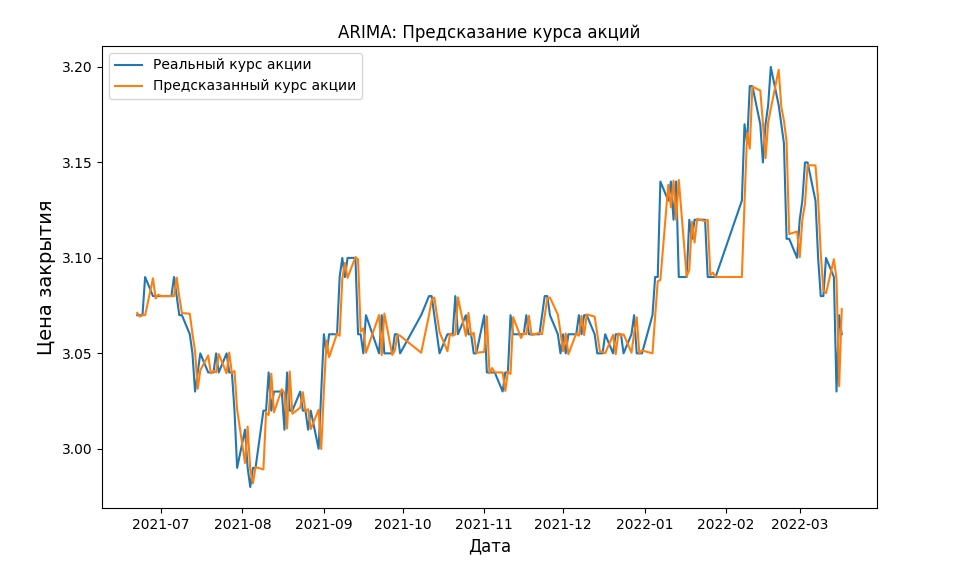
\includegraphics[width=0.8\textwidth]{img/arima.png}
  \caption{Предсказанный и реальный курс акций с использованием ARIMA.}
  \label{fig:research-arima}
\end{figure}

\par Остаток и плотность остатка предсказаний модели ARIMA показана на рисунке \ref{fig:residuals-and-density}.

\begin{figure}[hbtp]
  \centering
  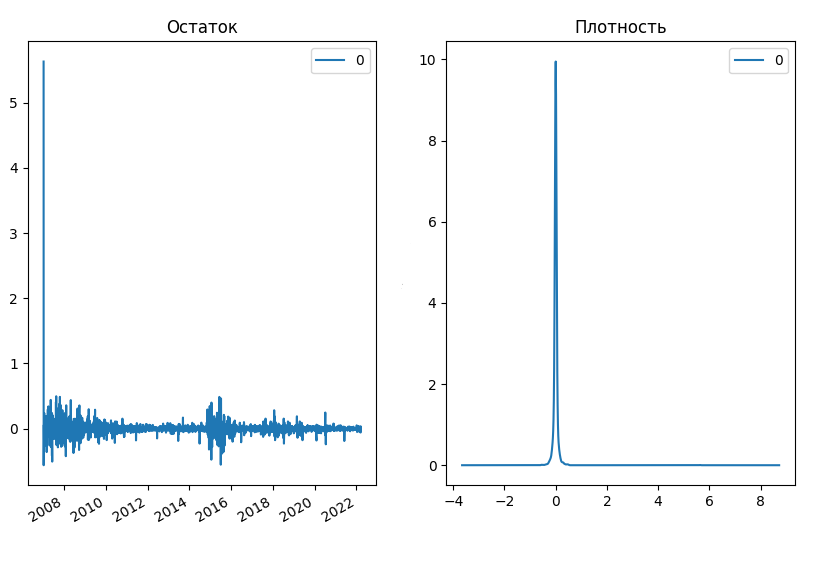
\includegraphics[width=\textwidth]{img/residuals_and_density.png}
  \caption{Остаток и плотность остатка предсказаний модели ARIMA.}
  \label{fig:residuals-and-density}
\end{figure}

\par Разница между предсказанным и реальным значением курса акций на обучающем и проверочном наборе отображена на рисунке \ref{fig:difffit}.

\begin{figure}[hbtp]
  \centering
  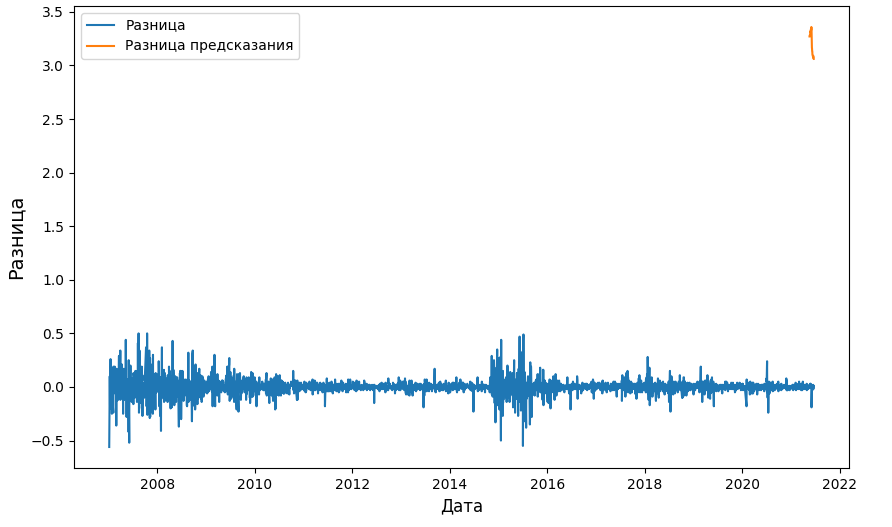
\includegraphics[width=\textwidth]{img/difffit.png}
  \caption{Разница предсказаний модели ARIMA.}
  \label{fig:difffit}
\end{figure}

\newpage

\textbf{ARIMA + XGBoost}

\par Эффективность предсказаний курса акций при помощи классической модели ARIMA с дальнейшей обработкой XGBoost регрессором отображена на рисунке \ref{fig:arima+xboost2}.

\begin{figure}[hbtp]
  \centering
  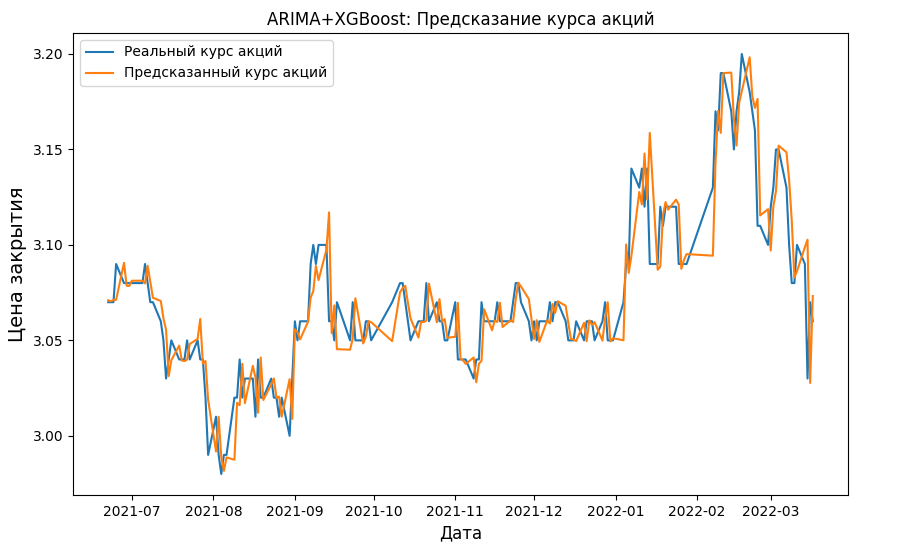
\includegraphics[width=0.7\textwidth]{img/arima+xboost2.png}
  \caption{Предсказанный и реальный курс акций моделью ARIMA+XGBoost.}
  \label{fig:arima+xboost2}
\end{figure}

\par Остаток предсказаний модели ARIMA + XGBoost показана на рисунке \ref{fig:arima+xboost}.

\begin{figure}[hbtp]
  \centering
  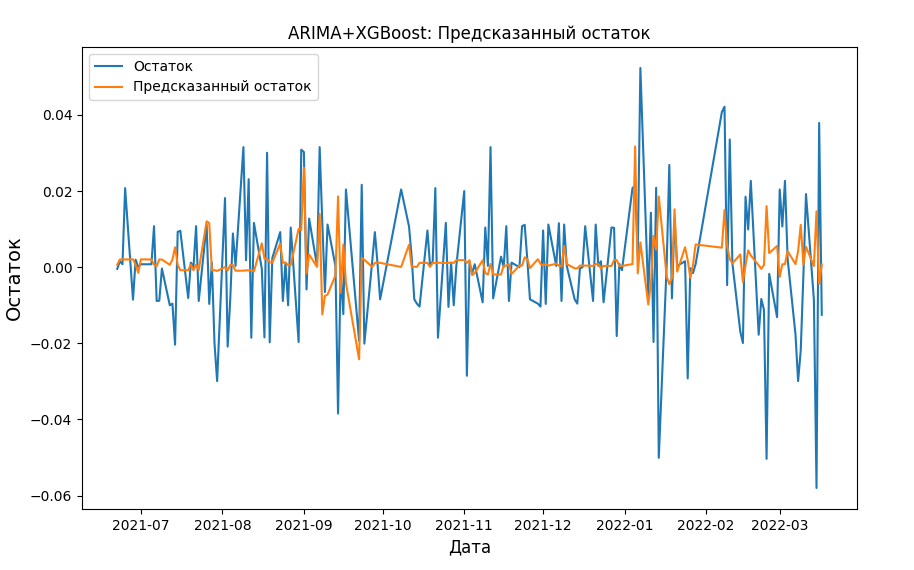
\includegraphics[width=0.7\textwidth]{img/arima+xboost.png}
  \caption{Остаток предсказанный моделью ARIMA + XGBoost.}
  \label{fig:arima+xboost}
\end{figure}

\newpage
\textbf{ARIMA + LSTM}

\par Кривые потерь исходной последовательности ARIMA + SingleLSTM показаны на рисунке \ref{fig:train-val-loss}.

\begin{figure}[hbtp]
  \centering
  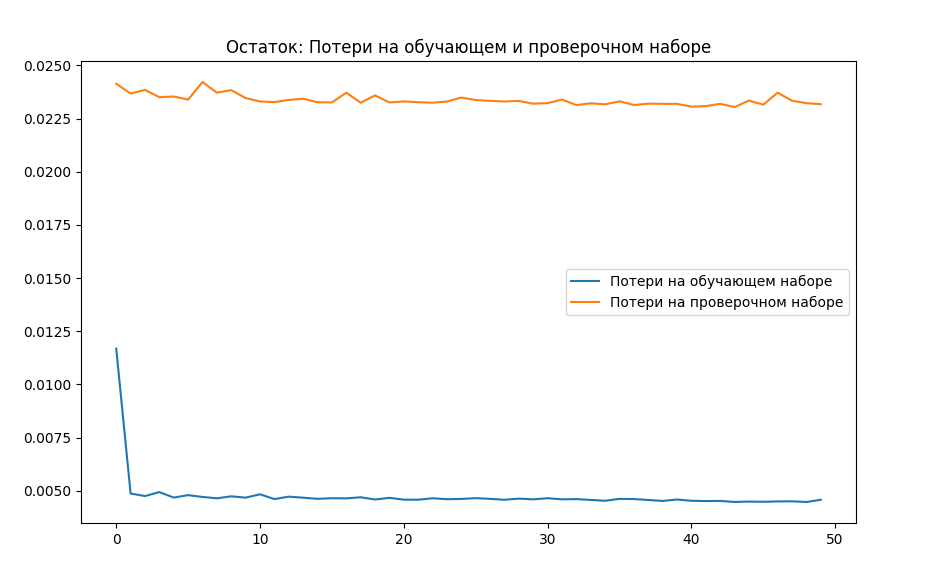
\includegraphics[width=0.75\textwidth]{img/train_val_loss.png}
  \caption{Потери исходной последовательности ARIMA + SingleLSTM.}
  \label{fig:train-val-loss}
\end{figure}

\par Кривые потерь остаточной последовательности ARIMA + SingleLSTM показаны на рисунке \ref{fig:lstm-train-val-loss}.

\begin{figure}[hbtp]
  \centering
  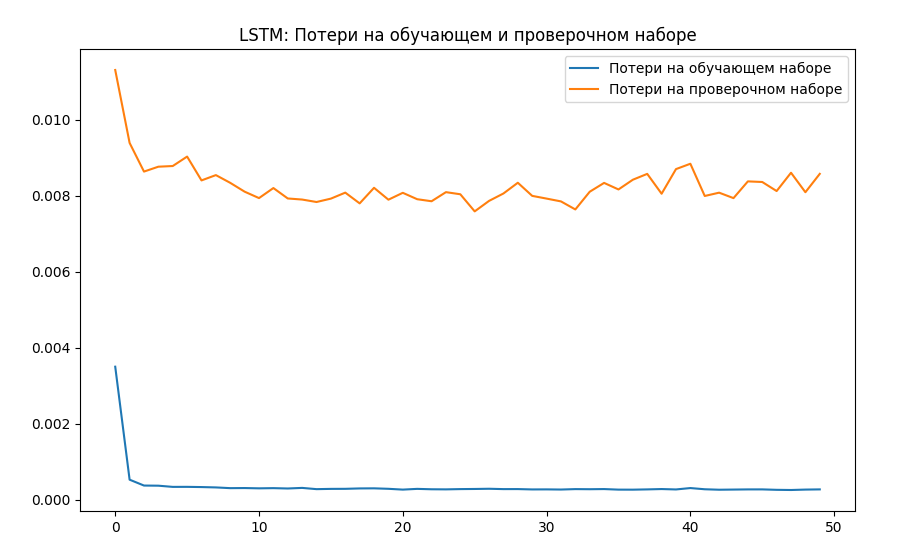
\includegraphics[width=0.75\textwidth]{img/lstm_train_val_loss.png}
  \caption{Потери остаточной последовательности ARIMA + SingleLSTM.}
  \label{fig:lstm-train-val-loss}
\end{figure}

\newpage
\par Эффективность предсказаний курса акций модели ARIMA + SingleLSTM отображены на рисунке \ref{fig:lstm}.

\begin{figure}[hbtp]
  \centering
  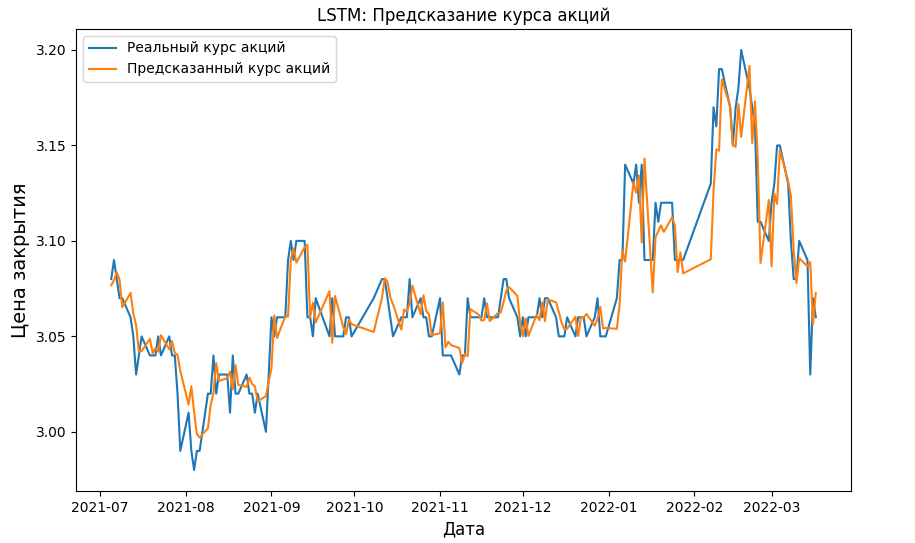
\includegraphics[width=0.78\textwidth]{img/lstm.png}
  \caption{Предсказанный курс акций моделью ARIMA + SingleLSTM.}
  \label{fig:lstm}
\end{figure}

\par Эффективность предсказания курса акций при помощи модели ARIMA + BiLSTM отображены на рисунке \ref{fig:bilstm}.

\begin{figure}[hbtp]
  \centering
  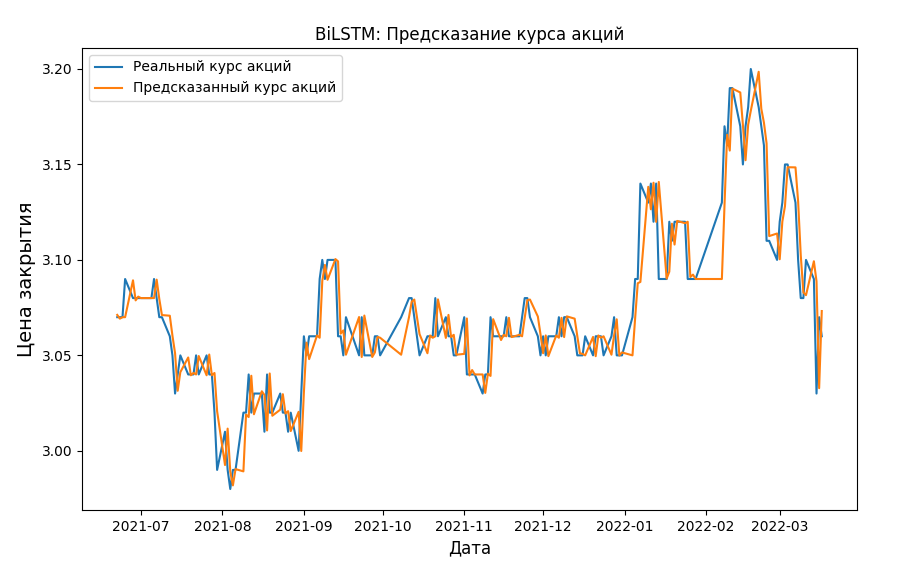
\includegraphics[width=0.78\textwidth]{img/bilstm.png}
  \caption{Предсказанный курс акций моделью ARIMA + BiLSTM.}
  \label{fig:bilstm}
\end{figure}

\newpage
\textbf{ARIMA + ACNN + LSTM + XGBoost}

\par Эффективность предсказания курса акций при помощи предложенной комбинированной модели ARIMA + ACNN + LSTM + XGBoost отображены на рисунке \ref{fig:hybrid-prediction}.

\begin{figure}[hbtp]
  \centering
  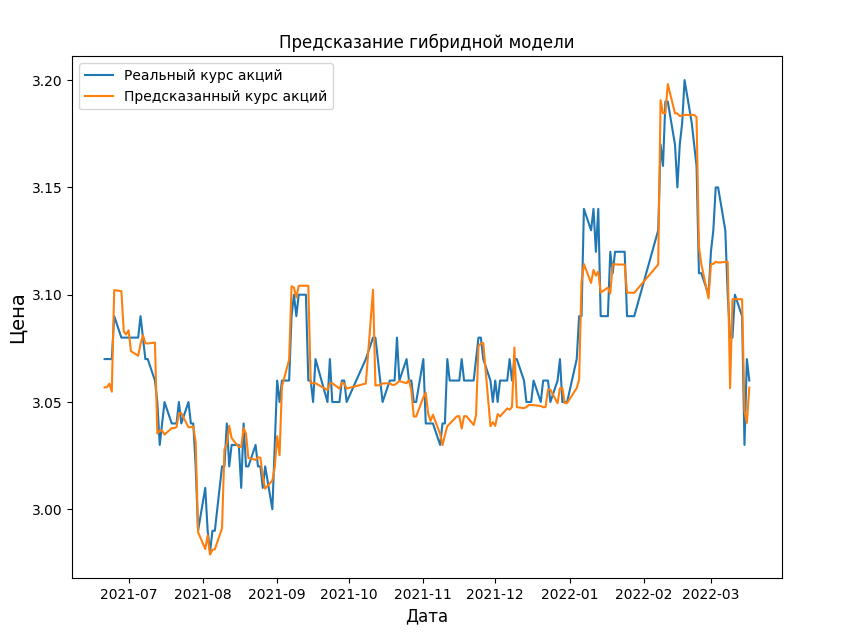
\includegraphics[width=\textwidth]{img/hybrid_prediction.png}
  \caption{Предсказанный курс акций гибридной моделью.}
  \label{fig:hybrid-prediction}
\end{figure}

\subsection{Сравнение комбинаций разработанных моделей}
\par Метриками оценки комбинации разработанных моделей будут служить: средняя абсолютная ошибка (MAE, формула \ref{eq:MAE}), корень среднеквадратичной ошибки (RMSE, формула \ref{eq:RMSE}), средняя абсолютная процентная ошибка (MAPE, формула \ref{eq:MAPE}), а также $R^{2}$, представленная в формуле \ref{eq:RR}.

\begin{equation}
    \label{eq:MAE}
    \text{MAE} = \frac{1}{n} \sum_{t=1}^{n} \left |\hat{X}_{t} - X_{t} \right |
\end{equation}

\newpage

\par Здесь $\bar{X_{t}}$ обозначает среднее значение $X_{t}$. Чем меньше ошибка и выше оценка $R^{2}$, тем лучше производительность соответственно.

\begin{equation}
    \label{eq:RMSE}
    \text{RMSE} = \sqrt{\frac{1}{n} \sum_{t=1}^{n} \left (\hat{X}_{t} - X_{t} \right )^{2}}
\end{equation}

\begin{equation}
    \label{eq:MAPE}
    \text{MAPE} = \frac{1}{n} \sum_{t=1}^{n} \left |\frac{\hat{X}_{t} - X_{t}}{X_{t}} \right |
\end{equation}

\begin{equation}
    \label{eq:RR}
    R^{2} = \frac{\sum_{t=1}^{n} {\left \| \hat{X}_{t} - \bar{X_{t}} \right \|}^{2}}{\sum_{t=1}^{n} {\left \| {X}_{t} - \bar{X_{t}} \right \|}^{2}} 
\end{equation}

\begin{table}[hbtp]
	\centering
	\caption{Сравнение различных сочетаний моделей предобучения-дообучения}
	\label{tab:comparsion}
	\resizebox{0.7\textwidth}{!}{%
		\begin{tabular}{|l|l|l|l|l|l|}
			\hline
			\textbf{Предобучение} & \textbf{Дообучение} & \textbf{MSE} & \textbf{RMSE} & \textbf{MAE} &  \textbf{R2}  \\ \hline
            \text{---}    &    \text{---}   &    0.00057     &   0.02734     &   0.02368 &   0.74402  \\ \hline
            \text{---}    &   \text{XGBoost} &    0.00031    &   0.01755     &   0.01223 &    0.82405  \\ \hline
            \text{SL-LSTM}     &   \text{SL-LSTM}     &   0.00045 &    0.02282    &   0.01960     &    0.79434   \\ \hline
            \text{ML-LSTM}     &   \text{ML-LSTM}    &    0.00031    &    0.01720    &    0.01265    &    0.82351   \\ \hline
            \text{BiLSTM}   &  \text{BiLSTM}  &   0.00027     &   0.01652     &    0.01201     &   0.84210   \\ \hline
            \text{BiLSTM}  &   \text{XGBoost}     &    0.00024     &  0.01605     & 0.01187   &   0.86301   \\ \hline
            \text{CNN-BiLSTM}  &   \text{XGBoost}     &   0.00022     &    0.01529    &    0.01145     &  0.87720    \\ \hline
            \text{ACNN-BiLSTM}     &   \text{XGBoost}  &  \textbf{0.00020}     &   \textbf{0.01424}     &    \textbf{0.01126}    &    \textbf{0.88342}  \\ \hline
		\end{tabular}%
	}
\end{table}

\subsection{Выводы из исследовательского раздела}

\par На основе проведенного исследования эффективности прогнозирования временных рядов при различных сочетаний моделей предобучения-дообучения можно утверждать, что разработанная концепция комбинированной модели \\ 
превосходит, как и отдельно взятые авторегрессионые и нейросетевые аналоги, так и их простейшие комбинации.


\pagebreak